\documentclass[11pt]{article}            % Report class in 11 points
\parindent0pt  \parskip10pt             % make block paragraphs
\usepackage{graphicx}
\usepackage{listings}
\graphicspath{ {images/} }
\usepackage{graphicx} %  graphics header file
\begin{document}
\begin{titlepage}
    \centering
  \vfill
    
\includegraphics[width=8cm]{uni_logo.png} \\ 
	\vskip2cm
    {\bfseries\Large
	Data Structures and algorythm  \\ (CS09203)\\
	
	\vskip2cm
	Lab Report 
	 
	\vskip2cm
	}    

\begin{center}
\begin{tabular}{ l l  } 

Name: & MuhammadTalhaKhalid \\ 
Registration \#: &CSU-S16-135\\ 
Lab Report \#: & 2 \\ 
 Dated:& 13-04-2018\\ 
Submitted To:& Mr. Usman Ahmed\\ 

 %\hline
\end{tabular}
\end{center}
    \vfill
    The University of Lahore, Islamabad Campus\\
Department of Computer Science \& Information Technology
\end{titlepage}


    
    {\bfseries\Large
\centering
	Experiment \# 2 \\

Data entry into array using Que \\
	
	}    
 \vskip1cm
 \textbf {Objective}\\  To understand How to Handle data into array  using Que.
 
 \textbf {Software Tool} \\
1. Ubuntu Linux \\
2. Sublime text\\
3. G++ \\

\section{Theory }              
In this experiment we learn how to handle our data in an array using The concept of Que,  and  learn the basics of  Link listing in c++ using Que.\\
It has 2 rules:\\
1.	Front should not be equal to rear.\\
2.	Your data should not reach the max  size of your array  .\\ \\
\section{Task}  
\subsection{Procedure: Task 1 }     

\begin{figure*}
\centering
  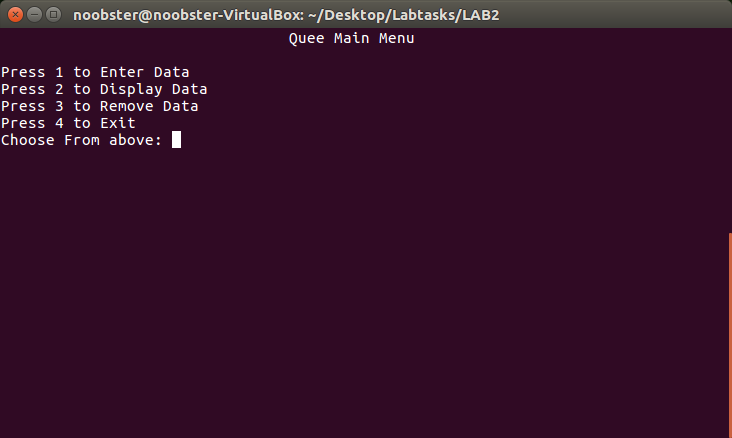
\includegraphics[width=12cm,height=6cm,keepaspectratio]{1.png}
\caption{Main menu of my program}
\label{Figure:1}    
  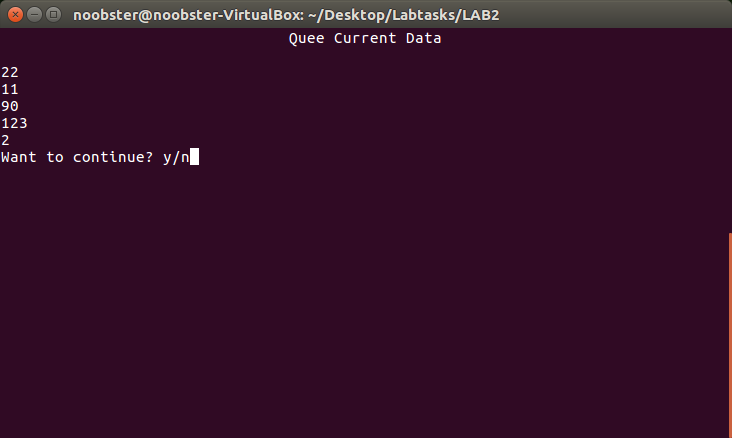
\includegraphics[width=12cm,height=6cm,keepaspectratio]{2.png}
\caption{New entry into array using Que}
\label{Figure:2}   
\end{figure*}
In this We enter our data into an  array  which contains  3 numbers
\subsection{Procedure: Task 2 }     
\begin{lstlisting}[language=C++]
#include<iostream>
#include<stdio.h>
#include <unistd.h>
#include<cstdlib>
#define SIZE 5
using namespace std;
int Data[SIZE];
int front=-1;
int rear=-1;
void Enter(int m) {
	if(rear>4) {
		cerr<<"Que is full!!\n";
		front=rear=-1;
	}else {
		Data[++rear]=m;
		cout<<"\nSucessfully Entered your data!!\n";
	}
}

void Delete() {
	if(front==rear) {
		cerr<<"Quee is Empty!!\n";
	}else {
		cout<<"Deleted  "<<Data[++front]<<endl;
	}
}

 void display()
               {
                   if(rear==front)
                     {
                          cout <<" queue empty\n";
                          return;
                     }
                   for(int i=front+1;i<=rear;i++)
                   cout <<Data[i]<<"\n";
               }
void list() {
	cout<<"\t\t\t\tQuee Main Menu\n\n";
	cout<<"Press 1 to Enter Data\n";
	cout<<"Press 2 to Display Data\n";
	cout<<"Press 3 to Remove Data\n";
	cout<<"Press 4 to Exit\n";
}
int choice;
string Ask="y";
int input;
int main() 
{
	do {
system("clear");
list();
cout<<"Choose From above: ";
cin>>choice;
switch (choice){
	case 1:
	do {
		system("clear");
	cout<<"\t\t\t\tQuee Data Entry\n\n";
	cout<<"Enter a number: ";
	cin>>input;
	Enter(input);
	cout<<"Want to continue? y/n";
	cin>>Ask;
		}while(Ask!="n");
	break;
	case 2:
	do {
		system("clear");
	cout<<"\t\t\t\tQuee Current Data\n\n";
	display();
	cout<<"Want to continue? y/n";
	cin>>Ask;
		}while(Ask!="n");
	break;
	case 3:
	do {
				system("clear");
	cout<<"\t\t\t\tQuee Remove data\n\n";
	Delete();
	cout<<"Want to continue? y/n";
	cin>>Ask;
		}while(Ask!="n");
	break;
	}
}while(choice!=4);
return 0;
}
\end{lstlisting}
\begin{figure*}
\section{Output: }
\centering
  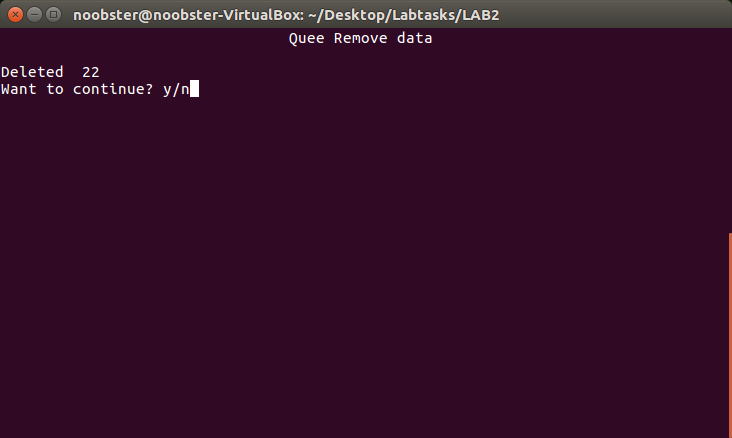
\includegraphics[width=12cm,height=6cm,keepaspectratio]{3.png}
\caption{Display output of my Stored Data}
\label{Figure:3}   
 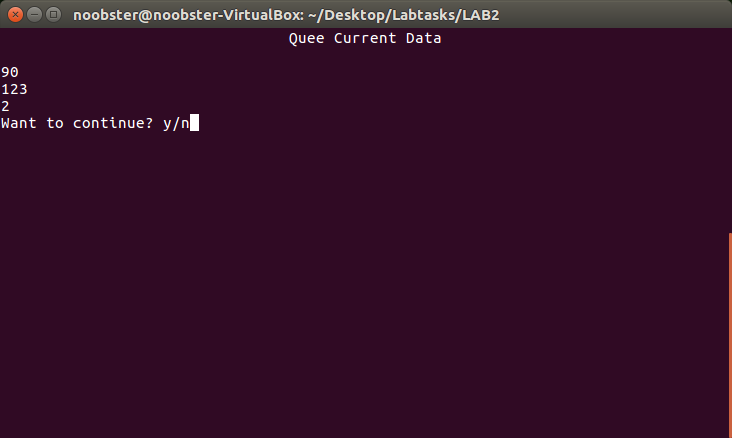
\includegraphics[width=12cm,height=6cm,keepaspectratio]{4.png}
\caption{Replace no array loacation Bilal With Junaid}
\label{Figure:4}
\end{figure*}
\begin{figure*}
 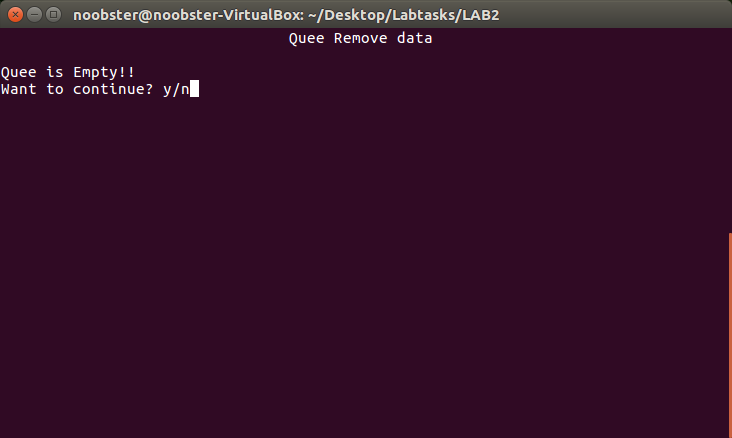
\includegraphics[width=12cm,height=6cm,keepaspectratio]{5.png}
\caption{Replaced Bilal with junaid in arrray location 2}
\label{Figure:5}
\section{Conclusion:}  
So In this Program we come to conclusion how to Handle our data into array using Que.  \\
Concept of front and rear in Que the two way process  \\
\end{figure*}

\end{document}                          % The required last line
